This section starts with the justification of why we choose Julia to implement the algorithm. Next, we describe the design of the interface of the algorithm. Then, we show a high-level design of the numerical software and present implementation details. Finally, we briefly compare the GSVD available in other numerical platforms. 

\subsection{Why Julia?}
There long exists a ``two-language'' problem programming language designers and software developers need to face: they have to make a trade-off when designing or choosing a language -- it can either be relatively easy for humans to write, or relatively easy for computers to run, but not both. \cite{perkel2019julia}

When it comes to the realm of numerical and scientific computing, the first language Fortran dated back to 1957. Over six decades, the landscape of computing has changed dramatically due to the advance of hardware, algorithms, and tremendous increased amount of data, among others. An unfortunate outcome is that the most challenging areas of scientific computing have benefited the least from the enhanced abstraction and productivity offered by higher-level languages. Modern scientific computing environments such as Python (Numpy)\cite{van2011numpy}, R \cite{ihaka1996r}, Mathematica \cite{math}, and MATLAB \cite{MATLAB}, to name a few, have grown in popularity and fall under the general category known as dynamic languages or dynamically typed languages. Still, when it comes to performance, C and Fortran remain the de facto for solving computationally intensive problems, especially in large scale. 

Fortunately, there is a new language, Julia, that aims to address this problem. Julia’s innovation lies exactly in the combination of productivity and performance. \cite{bezanson2017julia} Julia programming language fulfills much of the Fortran dream: automatic translation of formulas into efficient executable code. This means that by making use of JIT compilation, Julia can generate optimized native code for multiple architectures and can approach the speed of Fortran and C. On top of that, it allows programmers to write clear, high-level, generic and abstract code that closely resembles mathematical formulas, yet produces fast, low-level machine code that has traditionally only been generated by static languages.

\paragraph{Fast speed.} Some may think Julia is fast solely because it is Just-In-Time (JIT) compiled (i.e. every statement is run using compiled functions which are either compiled right before they are used, or cached compilations from before). However, other scripting languages Python, R, and MATLAB also use JIT, some by default. This leads to the question that what makes the key difference between Julia and other scripting languages in terms of speed?

The core design decision, type-stability through specialization via multiple-dispatch is what allows Julia to be very easy for a compiler to make into efficient code, but also allow the code to be very concise and "look like a scripting language". This will lead to some very clear performance gains. Multiple dispatch is the practice of having a function behave differently according to the number and the type of the parameters which it receives. It allows a language to dispatch function calls onto type-stable functions. If a function is type-stable, then the compiler can know what the type will be at all points in the function and smartly optimize it to the same assembly as C/Fortran.

\paragraph{Expressiveness.} MATLAB users may find a smooth transition to Julia as a fair amount of syntax of Julia are similar to that of MATLAB, if not the same. To begin with, both Julia and MATLAB use $\texttt{end}$ keyword to indicate code block. What's more, thanks to the magic of multiple dispatch, Julia brings ease of use to its programmers. Specifically, elementary operations are intuitive, as simple as math. 

	  \begin{table}[H]
        \centering
        \begin{tabular}{|| c | c | c ||} 
         \hline
         Operator & Function & Operand \\ [0.5ex] 
         \hline\hline
         \texttt{+} & add numbers/vectors/matrices & \makecell{\texttt{Int, Float, Vector, }\\ \texttt{Abstract Matrix, Dense Matrix, $\cdots$}} \\ \hline
         \texttt{*} & multiply scale or compose & \texttt{Number, Function} \\
         \hline\hline
        \end{tabular}
        \label{add-mul}
      \end{table}
        
\paragraph{A powerful approach to linear algebra.}
Besides support for multi-dimensional arrays, Julia provides native implementations for many linear algebra operations in the \texttt{LinearAlgebra} module. Basic matrix operations are implemented with calls to BLAS and LAPACK routines; the default implementation is OpenBLAS. Optimization efforts are also made in compact storage. For instance, QR decomposition may return a ``thin'' \texttt{R} matrix, which is stored in a compact blocked format. Furthermore, Julia users can easily write user-extensible wrappers for BLAS and LAPACK on top of the \texttt{LinearAlgebra} library. LAPACK wrappers are implemented fully in Julia code, using \texttt{ccall}, which does not require a C compiler. 

For example, in linear algebra, MATLAB programmers may first find Julia more friendly because the array index in Julia also starts at 1, not 0. Those who are familiar with MATLAB functions should quickly adapt new adventure in Julia. The table below summarizes a list of Julia commands for frequently used matrix decompositions, and their counterparts in MATLAB. 

	\begin{table}[H]
        \centering
        \scalebox{0.75}{
        \begin{tabular}{|| c | c | c ||} 
         \hline
         Julia command & MATLAB command & Description \\ [0.5ex] 
         \hline\hline
         \texttt{schur(A::StridedMatrix) -> F::Schur} & \texttt{T = schur(A)} & Schur decomposition \\ \hline
         \texttt{lu(A, pivot=Val(true); check = true) -> F::LU} & \texttt{[L,U] = lu(A)} & LU decomposition \\ \hline
         \texttt{qr(A, pivot=Val(false)) -> F} & \texttt{[Q,R] = qr(A)} & QR decomposition \\ \hline
         \texttt{eigen(A; permute::Bool=true, scale::Bool=true, sortby) -> Eigen} & \texttt{[V,D] = eig(A)} & Eigenvalues and eigenvectors \\ \hline
         \texttt{svd(A; full::Bool = false) -> SVD} & \texttt{[U,S,V] = svd(A)} & Singular value decomposition \\
         \hline\hline
        \end{tabular}
        }
        \caption{Interfaces of commonly seen matrix decompositions in Julia and MATLAB}
        \label{freq-decomp}
      \end{table}

In light of this, we implement the algorithm to compute the GSVD described in the previous section in Julia 1.3.

\Red{Where to put some potential issues?}

Meanwhile, we also capture some pitfalls that might be a bottleneck, and thus are worth mentioning.
\paragraph{Some inconsistent interface design.}
As a modern programming language, Julia supports multiple dispatch, that is, parametric polymorphism. A good example is that the GSVD interface reuses the name of the SVD of a single matrix $A$ by taking two matrices as arguments. Unfortunately, this principle is not fully implemented. For instance, when computing the matrix norm, one may intuitively call \texttt{norm(A)}. However, this will not produce the desired result as shown below. Instead, one may want to use \texttt{opnorm(A)}. 

		\begin{table}[H]
        \centering
        \begin{tabular}{|| c | c ||} 
         \hline
         Julia command/result & MATLAB command/result\\ [0.5ex] 
         \hline\hline
         \makecell{\texttt{norm([1 2 3; 4 5 6; 7 8 9])} \\
		 16.881943016134134} & \makecell{\texttt{norm([1 2 3;4 5 6;7 8 9])} \\ 16.8481} \\
		 \hline\hline
         \makecell{\texttt{opnorm([1 2 3; 4 5 6; 7 8 9])} \\
		 16.84810335261421} & N/A \\
         \hline\hline
        \end{tabular}
        \label{norm-api}
        \end{table}


\paragraph{Performance relies on ``proper'' implementation.}
Our GSVD algorithm involves many operations with submatrices. We don't need to pay attention to matrix slicing in other languages. However, in Julia, this could be a significant performance issue since slicing an array creates a copy of the selected subarray, which is computational expensive.  
To make things worse, if a sliced matrix is passed as the return value, the result will be inaccurate as it is not overwritten in the original matrix. 

An alternative is to create a ``view'' of the array, which is an array object that actually references the data of the original array in-place, without making a copy. This can be done for individual slices by calling function \texttt{view}, or more simply for a whole expression or block of code by putting macro \texttt{@views} in front of that expression. One can tell from the following example that by doing so, the speedup is three-fold. 
\begin{lstlisting}[language=julia, style=jlcodestyle]
	julia> fcopy(x) = sum(x[2:end-1]);

	julia> @views fview(x) = sum(x[2:end-1]);

	julia> x = rand(10^6);

	julia> @time fcopy(x);
  	0.003051 seconds (7 allocations: 7.630 MB)

	julia> @time fview(x);
  	0.001020 seconds (6 allocations: 224 bytes)
\end{lstlisting}

Many other features have not been studied and explored by the author, most notably, parallelism. This could be a good direction for future work. 

\subsection{Interface}
The products of the GSVD are six matrices and two integers indicating the rank information. To follow Julia's convention as an object-oriented language, we encapsulate all the products into a composite type named \texttt{GeneralizedSVD}. In this way, users do not need to explicitly enumerate every matrix or integer in the return statement. In addition, doing so will facilitate those who only want to access part of the products. Hence, we define the composite type as a struct. 

\begin{lstlisting}[language=julia, style=jlcodestyle]
struct GeneralizedSVD{T} <: Factorization{T}
    U::AbstractMatrix{T}
    V::AbstractMatrix{T}
    Q::AbstractMatrix{T}
    C::AbstractMatrix{T}
    S::AbstractMatrix{T}
    k::Int
    l::Int
    R::AbstractMatrix{T}
end
\end{lstlisting}

In the nineties, the cost of computer storage was a great concern in computational efforts. Thus, mostly of the LAPACK routines overwrite input matrices or vectors as outputs. Nowadays, computers are made much more cheaper, but the communication cost between memory and cache remains a bottleneck for numerical computing. Functions in Julia, particularly in ``\texttt{LinearAlgebra}'' package, are two-fold: one makes a copy of the input matrices or vectors, the other overwrite the inputs to save space. Now, we are ready to present the two interfaces.

\paragraph{Interface 1.} We adopt the practice of polymorphism when designing the interface of the GSVD. This enables SVD of one matrix and GSVD of a matrix pair to share a single interface with entities of different number of input parameters. Such polymorphism allows a function to be written generically and thus maintain the language's expressiveness. 

\newpage

\begin{lstlisting}[language=julia, style=jlcodestyle]
svd(A, B) -> GeneralizedSVD
\end{lstlisting}

Compute the generalized SVD of \texttt{A} and \texttt{B}, returning a \texttt{GeneralizedSVD} factorization object \texttt{F}, such that \texttt{A = F.U*F.C*F.R*F.Q'} and \texttt{B = F.V*F.S*F.R*F.Q'}. \\

For an m-by-n matrix \texttt{A} and p-by-n matrix \texttt{B},

    \begin{itemize}
        \item \texttt{U} is an m-by-m orthogonal matrix,
        \item \texttt{V} is a p-by-p orthogonal matrix,
        \item \texttt{Q} is an n-by-n orthogonal matrix,
        \item \texttt{C} is an m-by-(k+l) diagonal matrix with 1s in the first K entries,
        \item \texttt{S} is a p-by-(k+l) matrix whose top right L-by-L block is diagonal,
        \item \texttt{R} is a (k+l)-by-n matrix whose rightmost (k+l)-by-(k+l) block is nonsingular upper block triangular,
        \item \texttt{k+l} is the effective numerical rank of the matrix \texttt{[A; B]}.
    \end{itemize}
    
Iterating the decomposition produces the components \texttt{U, V, Q, C, S, and R}. 

\paragraph{Interface 2.} We provide another interface that overrides input matrices. 

\begin{lstlisting}[language=julia, style=jlcodestyle]
svd!(A, B) -> GeneralizedSVD
\end{lstlisting}

\texttt{svd!} is the same as \texttt{svd}, but modifies the arguments \texttt{A} and \texttt{B} in-place, instead of making copies. It returns a \texttt{GeneralizedSVD} factorization object \texttt{F}, such that \texttt{A = F.U*F.C*F.R*F.Q'} and \\ 
\texttt{B = F.V*F.S*F.R*F.Q'}. \\
 
For an m-by-n matrix \texttt{A} and p-by-n matrix \texttt{B},

    \begin{itemize}
        \item \texttt{U} is an m-by-m orthogonal matrix,
        \item \texttt{V} is a p-by-p orthogonal matrix,
        \item \texttt{Q} is an n-by-n orthogonal matrix,
        \item \texttt{C} is an m-by-(k+l) diagonal matrix with 1s in the first K entries,
        \item \texttt{S} is a p-by-(k+l) matrix whose top right L-by-L block is diagonal,
        \item \texttt{R} is a (k+l)-by-n matrix whose rightmost (k+l)-by-(k+l) block is nonsingular upper block triangular,
        \item \texttt{k+l} is the effective numerical rank of the matrix \texttt{[A; B]}.
    \end{itemize}
    
Iterating the decomposition produces the components \texttt{U, V, Q, C, S, and R}. 

\subsection{Design and implementation}
The structural unit called \texttt{Module} is native in Julia to group relevant functions and definitions. The main module is \texttt{GSVD}. Considering that the safe diagonalization not only serves as a building block for our GSVD algorithm, but is also a powerful tool in other applications, it is wise to separate safe diagonalization as a standalone module called \texttt{SafeDiag}. The high-level architecture of the GSVD software is shown in the UML class diagram below.

	\begin{figure}[H]
        \centering
        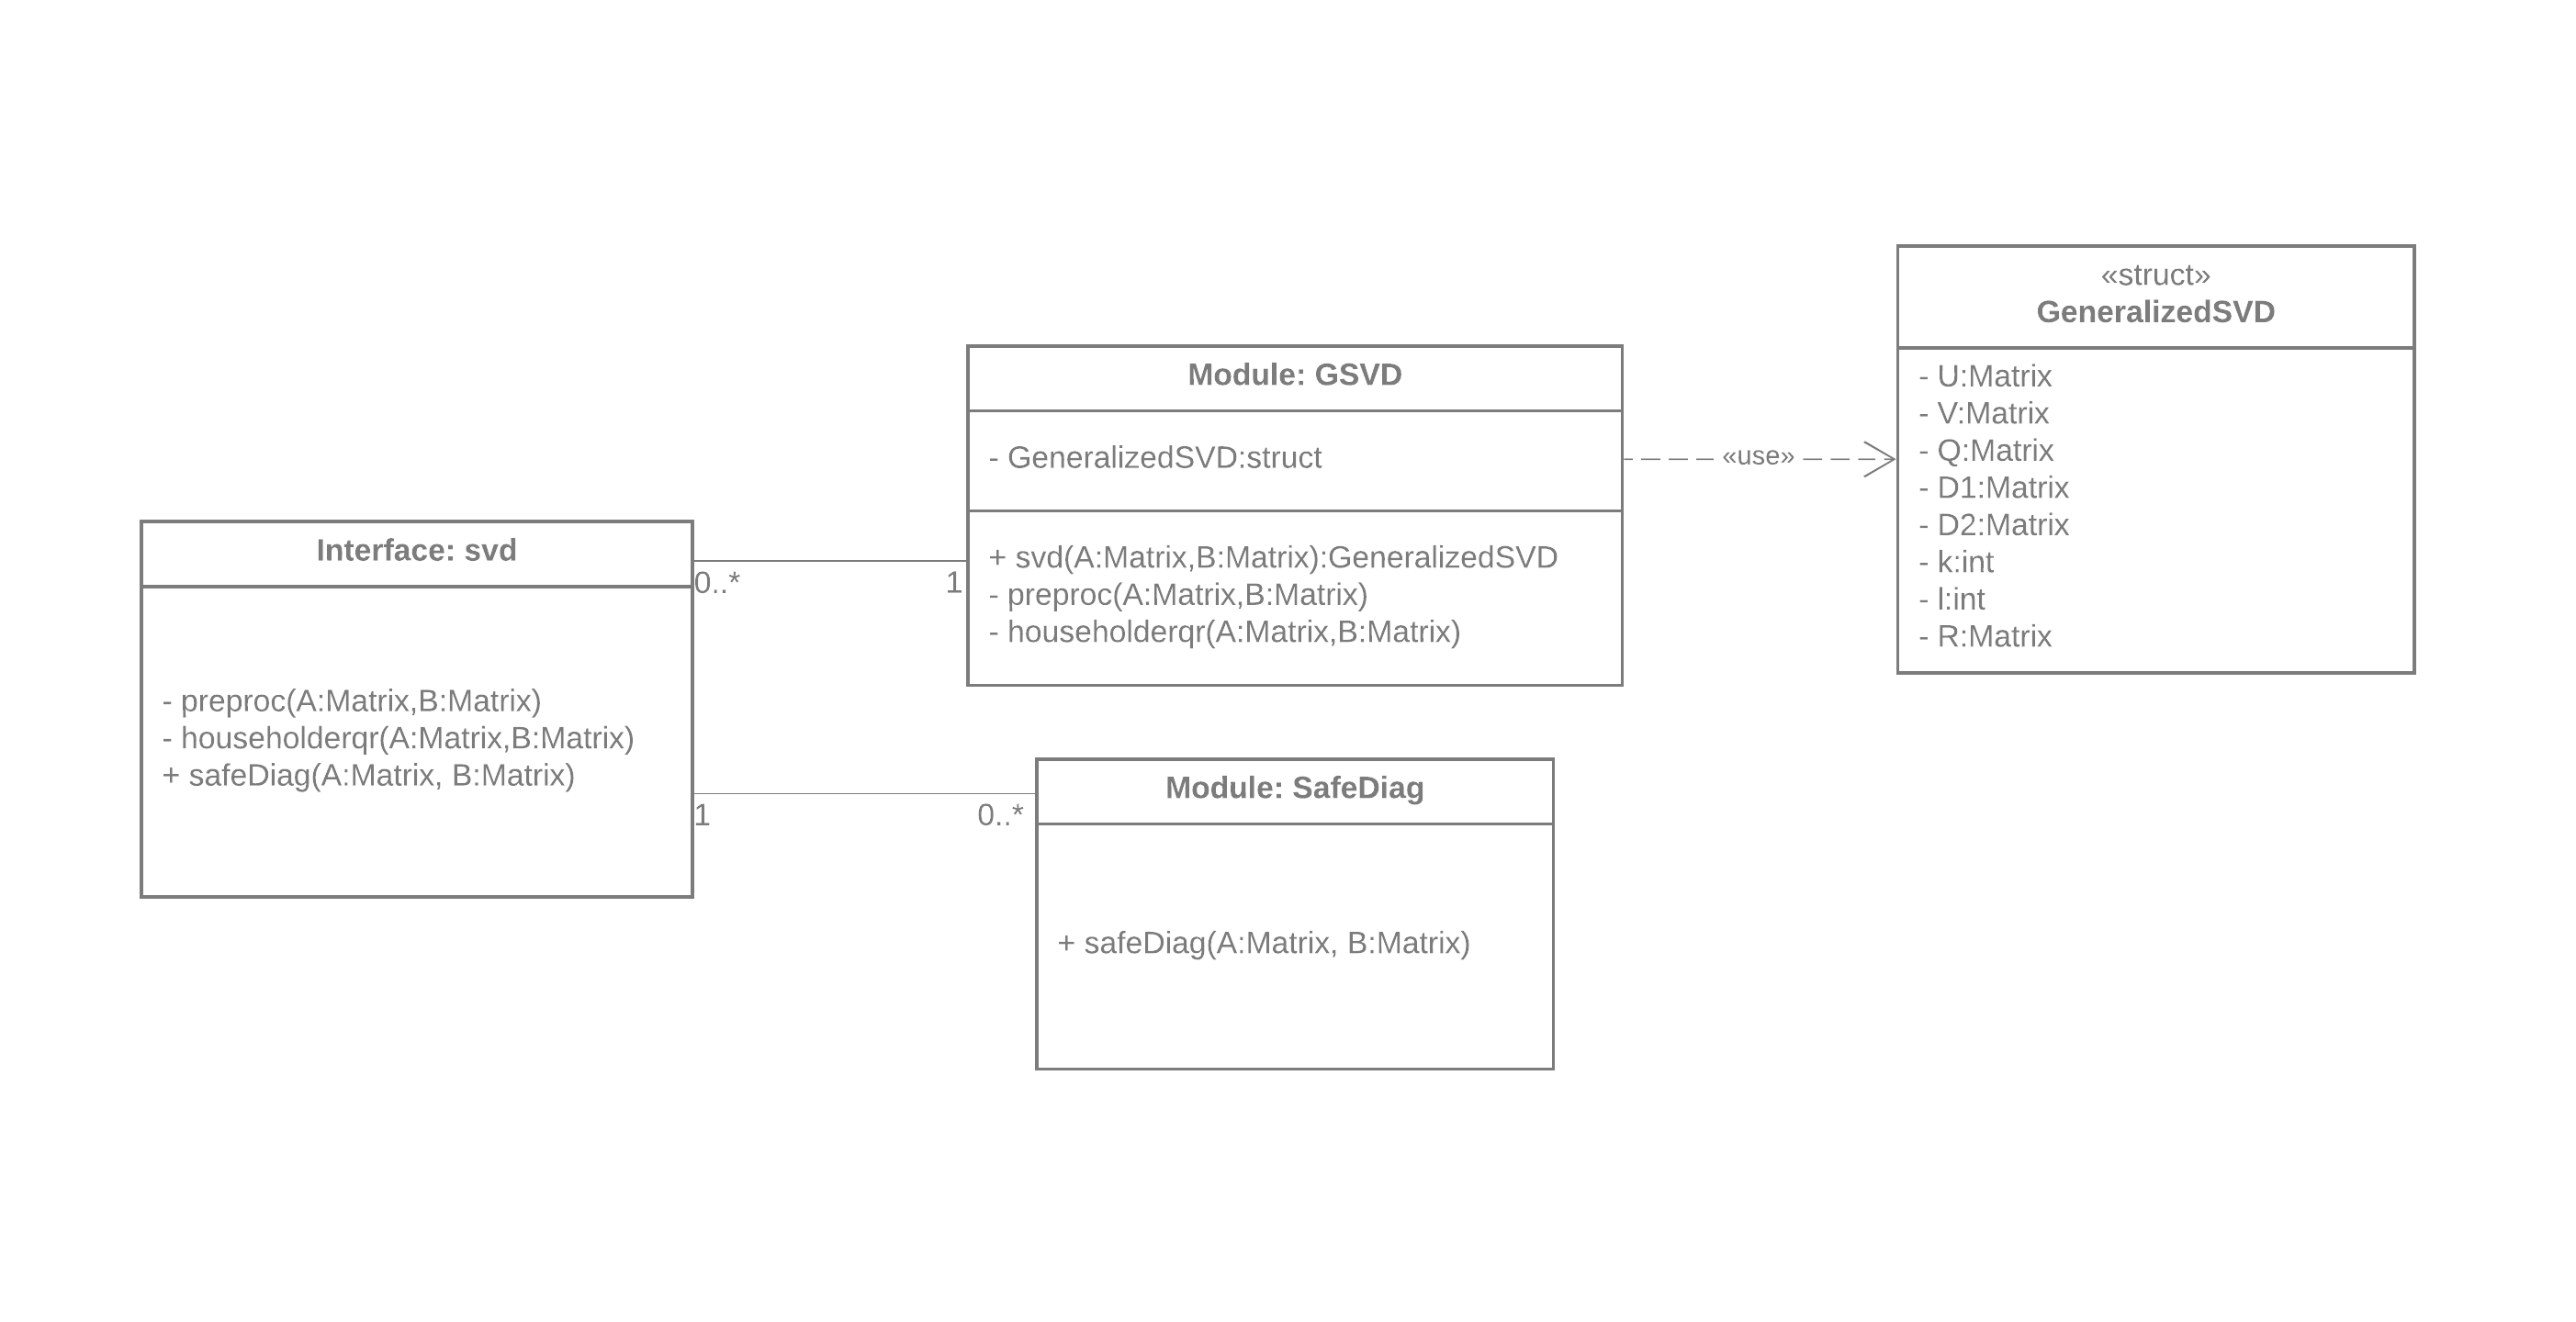
\includegraphics[width=0.75\linewidth]{fig/GSVD_class.png}
        \label{uml-class}
        \caption{UML class diagram for the GSVD}
    \end{figure}

According to the architecture design, the algorithm thus starts from the main function \texttt{svd()} under module \texttt{GSVD}. It then calls \texttt{preproc()}. Once return, it calls function \texttt{safeDiag} intermodularly. Finally, upon return, the main function post-processes to formulate the outputs. The sequence of the major function calls is the following. 

\begin{center}
    \fbox{\texttt{GSVD:svd()}} $\rightarrow$ \fbox{\texttt{GSVD:preproc()}} $\rightarrow$ \fbox{\texttt{GSVD:householderqr()}} $\rightarrow$ \fbox{\texttt{SafeDiag:safediag}}
\end{center}

We implement the GSVD algorithm described in the previous section in Julia 1.3 using \texttt{Float64} data. 

\begin{enumerate}[\textit{Step} 1]
    \item Pre-processing:
    
    This step is to reduce two input matrices $A$ and $B$ into two upper triangular forms. This is done via a call to \texttt{preproc()}. This function makes use of three fundamental orthogonal decompositions. 
    \begin{enumerate}
    	\item First is QR decomposition with column pivoting to reveal the numerical rank of $B$ and $[A; B]$ without forming the matrix explicitly. This is done by a call to \texttt{qr(A, pivot=Val(true)))}. Let \texttt{tolB} as the tolerance to determine the effective rank of $B = \ell$.
		\begin{equation*}
			tol_{B} = max\{p, n\}\Vert B \Vert_1 \epsilon
		\end{equation*}
		where $\epsilon$ is the machine precision of \texttt{Float64}. \\
		We also use QR decomposition with column pivoting again on the leftmost $n-\ell$ columns of $A$. Similarly, by defining
		\begin{equation*}
			tol_{A} = max\{m, n\}\Vert A \Vert_1 \epsilon
		\end{equation*}
		we compute the effective rank of $[A; B] = k+ \ell$.
		\item Second is RQ decomposition of the top $\ell$ rows of $B$ if $n > \ell$ via a call to \texttt{LAPACK.gerqf!()}. It is called a second time on $A$ if $n - \ell > k$.
		\item Third is QR decomposition of $A$ when $m > k$ by calling \texttt{qr()}. 
	\end{enumerate}
	Upon return to \texttt{svd()}, two of the upper triangular matrices overwrites $A$ and $B$, the orthogonal matrices are placed in U, V, and Q and rank information is stored in $k$ and $\ell$.
    \item QR decomposition:
    
    This step is to reduce two upper triangular matrices to one and is done by calling \texttt{householderqr()}. On entry, two triangular matrices are stacked together and passed as the arguments of \texttt{qr()}. On exit, $Q_1$ and $Q_2$ overwrites inputs.  
    
    \item Safe diagonalization:
    
    This step calls \texttt{safeDiag()} from module \texttt{SafeDiag}. This function requires SVD, and QR decomposition. This is done by calls to \texttt{svd()}, \texttt{qr()} respectively. 
    \begin{enumerate}
    	\item We first compute SVD of $Q_{2}$. To preserve the order of $\{\cos\theta\}$, we have to reverse the order of the singular values of $Q_{2}$. 
		\item Since $\{\cos\theta\}$ are already sorted, we take advantage of binary search to find the threshold $r$.
		\item QR decomposition of the multiply of $Q_{1}$ and right singular vectors of $Q_{2}$. $R$ is not only triangular but diagonal. However, sanitization is necessary to assure the non-negativity of the diagonal entries. 
    \end{enumerate}
    
    It return $U_1, V_1, Z_1, C, S$ on exit.   
    
    \item Post-processing:
    In this step, we update matrix $U$, $V$ and $Q$ by matrix-matrix multiply. To formulate $R$, we utilize RQ decomposition via a call to \texttt{LAPACK.gerqf!()}. Finally, we put matrices $U, V, C, S, Q$ and $k$, $\ell$ into the constructor of \texttt{GeneralizedSVD} as return. 
\end{enumerate}

\subsection{GSVD in other languages: a comparison}
    As we discussed at the beginning of this section, a number of numerical computing platforms feature the Generalized Singular Value decomposition. Here, we list several some of them and the corresponding documentation, shown in Table \ref{tab:gsvdlang}. 
    
    \begin{table}[H]
        \centering
        \begin{tabular}{|c|c|}
            \hline
            Language & GSVD Documentation \\ \hline\hline
            Native Julia (proposed) &  \makecell[l]{\texttt{svd(A, B) -> GeneralizedSVD} \\ Computes the generalized SVD of \texttt{A} and \texttt{B},  returning a \texttt{GSVD} factorization\\ object \texttt{F}, such that \\ \texttt{A = F.U*F.C*F.R*F.Q'} and \texttt{B = F.V*F.S*F.R*F.Q'}.}\\ \hline
            Julia 1.3 (LAPACK wrapper) &  \makecell[l]{\texttt{svd(A, B) -> GeneralizedSVD} \\ Computes the generalized SVD of \texttt{A} and \texttt{B},  returning a \texttt{GeneralizedSVD}\\ factorization object \texttt{F}, such that \\ \texttt{A = F.U*F.D1*F.R0*F.Q'} and \texttt{B = F.V*F.D2*F.R0*F.Q'}.}\\ \hline
            MATLAB (2019b) & \makecell[l]{\texttt{[U,V,X,C,S] = gsvd(A,B)} \\
            Returns unitary matrices \texttt{U} and \texttt{V}, a (usually) square matrix \texttt{X}, and \\ nonnegative diagonal matrices \texttt{C} and \texttt{S} so that \\
                \texttt{A = U*C*X', B = V*S*X', C'*C + S'*S = I}.}\\ \hline
            Mathematica & \makecell[l]{\texttt{SingularValueDecomposition[{m,a}]} \\
            Gives a list of matrices \{\texttt{{u,ua},{w,wa},v}\} such that \texttt{m} can be written as \\ \texttt{u.w.Conjugate[Transpose[v]]} and \texttt{a} can be written as \\ \texttt{ua.wa.Conjugate[Transpose[v]]}. } \\ \hline
            R (geigen v2.3, LAPACK wrapper) & \makecell[l]{\texttt{z <- gsvd(A, B)}\\
            Computes The Generalized Singular Value Decomposition of matrices \\ $A$ and $B$ such that $A = UD_{1}[0 \ R]Q^{T}$ and $B = VD_{2}[0 R]Q^{T}$. Note that \\ the return value is the same as the output of LAPACK 3.6 and above. }
            \\\hline
            Python (R. Luo's thesis) &  \makecell[l]{Didn't disclose API design. The author defined GSVD as follows: \\
            Given two $M_i$-by-$N$ column-matched but row-independent matrices $D_{i}$, \\ each with full column rank and $N \leq Mi$, the GSVD is an exact \\ simultaneous factorization $Di = Ui \Sigma_i V^T, i = 1, 2$. $U_i$ is $M_i$-by-$N$ and \\ are column-wise orthonormal and $V$ is $N$-by-$N$ nonsingular matrix with\\ normalized rows. $diag(\Sigma_i)$ returns two lists of $N$ positive values and \\the ratios are called the generalized singular values.} \\ \hline
        \end{tabular}
        \caption{GSVD in different languages}
        \label{tab:gsvdlang}
    \end{table}